\documentclass{prova}

\usepackage{amsmath}
\usepackage{amsfonts}

\setlength{\textheight}{25cm}

\renewcommand{\sin}{\,\mbox{sen}\,}
\newcommand{\ds}{\displaystyle}

\professor{Prof.\@ Adriano Barbosa}
\disciplina{C\'alculo Diferencial e Integral II}
\avaliacao{Final}
\curso{Qu\'{\i}mica}
\data{12/09/2023}

\begin{document}
	\cabecalho{5}  % o numero 5 indica a qnt de quadros na tabela de nota

    \textbf{Todas as respostas devem ser justificadas.}

    \begin{questionario}
        \q{Resolva a integral definida $\ds\int_1^{e} \frac{\sin{(\ln
           x)}}{x}\ dx$.}
        \q{Calcule a integral indefinida $\ds\int e^x x^2\ dx$.}
        \q{}
            \begin{questionario}
                \qq{Resolva a equa\c{c}\~ao $\ds 4y''+12y'+8y=0$.}
                \qq{Resolva o problema de valor inicial $\ds xy'+y=4x^2$,
                    $y(1)=0$.}
            \end{questionario}
        \q{Determine o maior intervalo aberto onde a s\'erie $\ds
            \sum_{n=0}^\infty \frac{2^n{(x-3)}^n}{\sqrt{n+3}}$ \'e convergente.}
        \q{Tri\^angulos ret\^angulos s\~ao construidos como na figura abaixo. Cada
           tri\^angulo tem altura 1 e sua base tem medida igual a hipotenusa do
           tri\^angulo anterior. Determine se a s\'erie $\ds\sum_{n=1}^\infty h_n$,
           formada pela soma das hipotenusas desses tri\^angulos, \'e convergente
           ou divergente.}
           \begin{figure}[h]
               \centering
               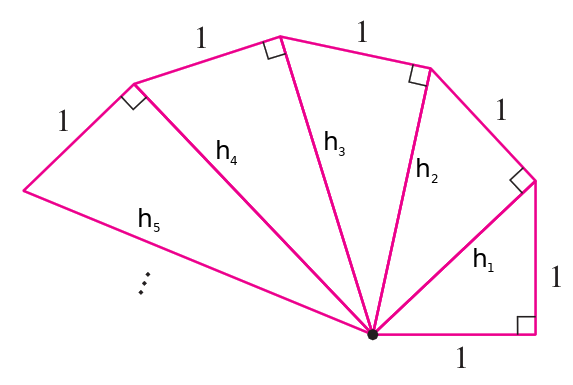
\includegraphics[width=0.5\textwidth]{triangulos.png}
           \end{figure}
    \end{questionario}
\end{document}
